\documentclass[a4paper]{article}

%\usepackage{fullpage} % Package to use full page
\usepackage{parskip} % Package to tweak paragraph skipping
\usepackage{tikz} % Package for drawing
\usepackage{amsmath}
\usepackage{hyperref}
\usepackage[T1]{fontenc}
\usepackage[utf8]{inputenc}
\usepackage[french]{babel}
\usepackage{wrapfig}

\title{1st week report}
\author{Reda YAHOU}
\date{\today}

\begin{document}

\maketitle

\section*{Introduction}

Ce document a pour but de résumer le travail qui a été réalisé durant la première semaine de stage. L'objectif de ce papier est principalement de synthétiser les concepts qui intervenant dans la trajectographie de fusée, ainsi, certaines notions physiques et mécaniques seront passées sous silence et seul l'essentiel sera mis en lumière.\\

Dans un premier temps vont être abordés et présentés les éléments de base nécessaire à la compréhension de la trajectographie de fusée. Par la suite sera établie un parallèle entre ces notions théoriques et le code de calcul Pégase : on verra comment le vol de fusée y est intégré ainsi que les étapes et les méthodes utilisées par cette interface pour la simulation. une dernier paragraphe viendra conclure ce rapport en introduisant au cas multi-étagé.\\


\begin{figure}[!htbp]
\begin{center}
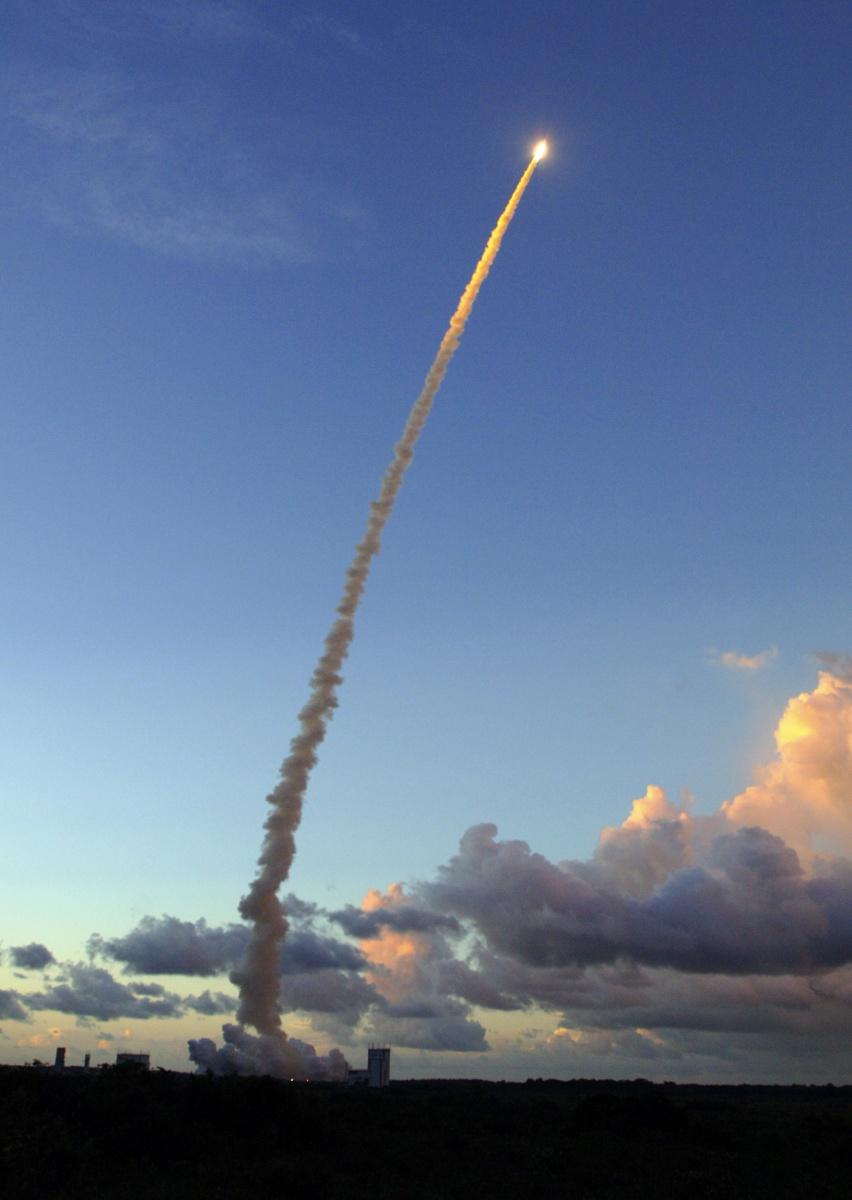
\includegraphics[width=4cm]{Kourou---Decollage-Ariane-5---V184.jpg} 
\end{center}
\caption{Kourou - Décollage d'Ariane 5.}
\end{figure}



\part{Trajectographie de fusée}

\section{Le vol de fusée}

En trajectographie, on décompose le vol de fusée en 3 grandes phases (voir schéma ci-dessous) : 

\begin{enumerate}
\item La phase propulsée
\item La phase balistique
\item La descente sous parachute
\end{enumerate}

\begin{figure}[!htbp]
\begin{center}
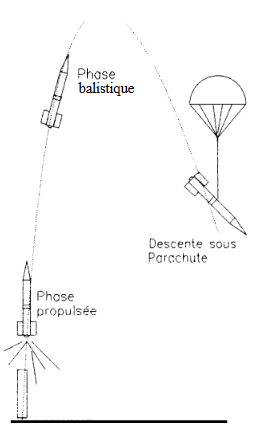
\includegraphics[width=3.5cm]{phases_vol.PNG} 
\end{center}
\caption{Les phases du vol.}
\end{figure}


\begin{enumerate}
\item Cette première phase s'écoulant  de  l'instant  de  la  mise à  feu à  la  fin  de  combustion  du  propulseur, comprend  une  partie  où  la  fusée  est  
guidée par la rampe de lancement et une partie où la fusée est livrée à elle-même. 
\item Après l'extinction du propulseur commence la  phase  balistique
  pendant  laquelle  la  fusée,  
uniquement soumise à son poids et à la résistance 
de l'air, exploite la vitesse acquise pendant la propulsion pour atteindre son altitude maximale. 
\item Une fois la culmination atteinte, lorsque l'engin commence à retomber, la phase balistique se 
poursuit  jusqu'à l'ouverture  du  parachute,  ce  qui  lui  permet  
de  revenir  au  sol  tout  en  
demeurant la plus intact possible. \\  
\end{enumerate} 


Pendant le vol d'une fusée, deux paramètres vont être étudié : 

\begin{itemize}

\item la simulation de sa trajectoire, c'est à dire l'allure de sa courbe, son altitude maximale, sa portée, le temps de vol. Ceci est entre autre modélisable à partir d'un système d'EDO.
\item la stabilité de la fusée.


\end{itemize}

La seconde notion soulève deux aspect : un aspect "esthétique", on désire avoir une belle courbe et un aspect sécuritaire.\\

En effet, au delà du fait d'obtenir la trajectoire d'une fusée, on souhaite aussi que cette dernière soit stable, c'est à dire qu'elle retrouve vite sa position initiale dés qu'elle se met en incidence.
Le paragraphe suivant aura pour objectif de détailler cette notion de stabilité.




\section{Stabilité de la fusée}



\paragraph{Les forces}
Pendant le vol, la fusée est soumise à trois forces : le Poids \textbf{$\vec P$}, la Poussée du moteur, \textbf{$\vec F$} et la résistance à l'air \textbf{$\vec R$}.

C'est la portance \textbf{$\vec R_{N}$}, composante normale de \textbf{$\vec R$}, qui va créer un moment et être responsable du mouvement de rotation. Elle va s'appliquer sur le centre de poussée dynamique \textbf{Cpa} et va dépendre de \textbf{$C_{N}\alpha$}, le coefficient de portance et du carré de la vitesse \textbf{$v^{2}$}. \\
\paragraph{Stabilité statique}



La distance entre le \textbf{Cpa} et le \textbf{Cdm} (Centre de masse) est appelé la \textbf{marge statique}.\\
La position du \textbf{Cpa} et \textbf{$C_{N}\alpha$} peuvent être déterminés grâce aux méthodes de Barrowmann, basées sur la géométrie des éléments de la fusée.\\
L'expérience montre que pour certains type de fusée, la stabilité dépend de la valeur de la marge statique i.e que la fusée est stable si la marge statique est  comprise dans un certain intervalle de valeur.\\
De manière similaire, le terme \textbf{$C_{N}\alpha$} va aussi influer sur la stabilité dans la mesure ou il intervient dans le moment de rotation provoquer par la portance : la fusée sera stable si la rotation est bien contrôlée.\\
D'un point de vie pratique, c'est les dimensions des ailes qui vont influer sur le facteur  \textbf{$C_{N}\alpha$}.


\begin{figure}[h!]
  \centering
  \begin{minipage}[b]{0.4\textwidth}
    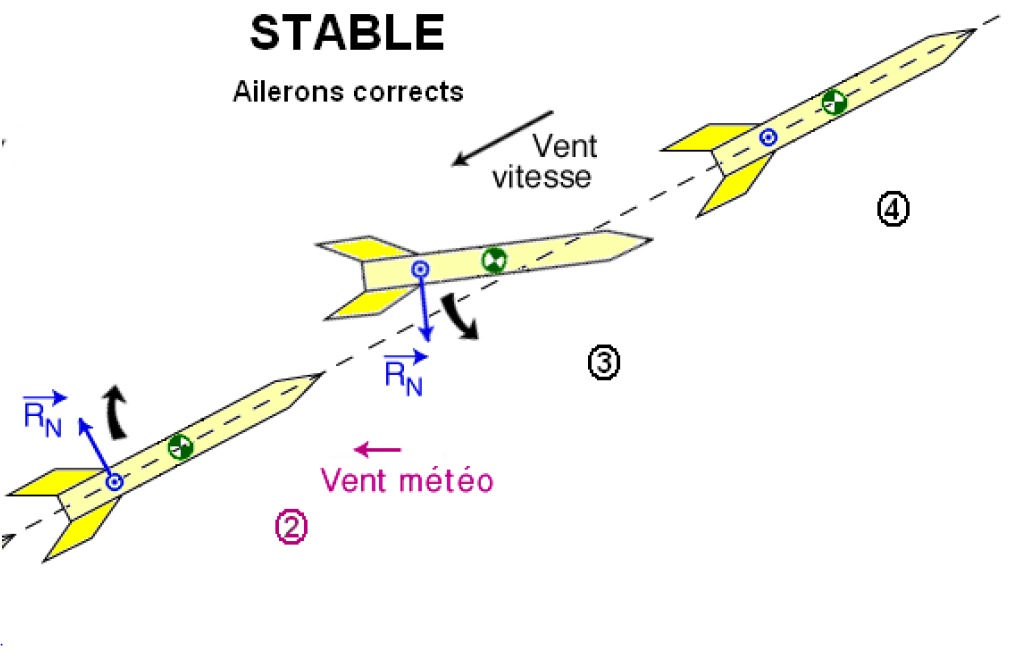
\includegraphics[width=\textwidth]{stable.png}
    \caption{Vol stable}
  \end{minipage}
  \hfill
  \begin{minipage}[b]{0.4\textwidth}
    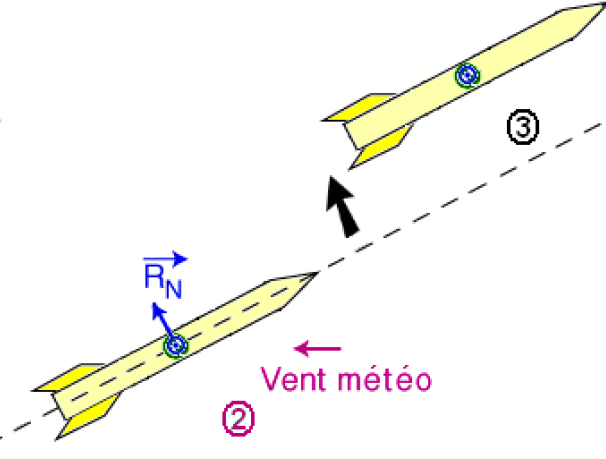
\includegraphics[width=\textwidth]{instable.png}
    \caption{Vol instable}
  \end{minipage}
\end{figure}

En pratique, la fusée est stable lorsque :
\begin{enumerate}
\item la marge statique est entre 1.5 est 7.
\item  \textbf{$C_{N}\alpha$} est comprise entre 15 et 30.
\item le produit de ces deux paramètres est entre 30 et 100.
\end{enumerate}



\paragraph{Stabilité dynamique}

Pendant le vol, la fusée va être soumise à des perturbation extérieur telles que le vent. Elles vont provoquer des oscillations chez cette dernière autour de sa position d'incidence nulle sources d'instabilités.\\

En pratique, ces oscillations vont décroitre : c'est le phénomène d'amortissement. Dans le cas stable, le ratio entre deux extremums dans les oscillations diminue jusqu'à que l'incidence soit nulle.

\begin{figure}[!htbp]
\begin{center}
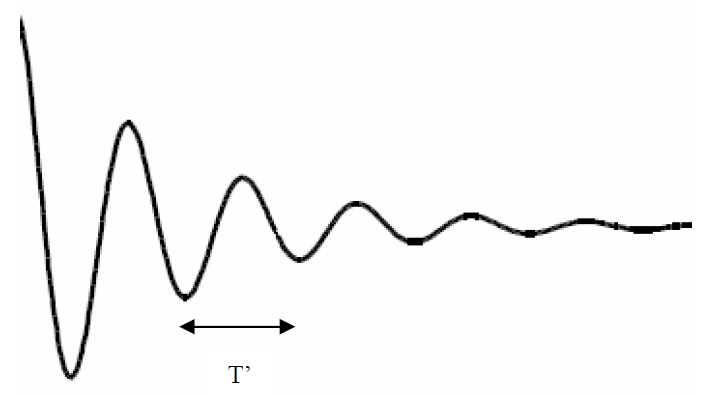
\includegraphics[width=5cm]{ammortissement.PNG} 
\end{center}
\caption{Évolution de l'incidence d'une fusée stable.}
\end{figure}

L'équation donnée par le Principe fondamentale de la dynamique en rotation donne : 

\begin{equation}
\frac{d^{2} \alpha}{dt^{2}} + 2\omega_{0} \xi  \frac{d \alpha}{dt} + \omega_{0}^{2}\alpha = 0
\end{equation}

Le terme $\xi$ représente le taux d'amortissement. D'un point de vue pratique, l'amortissement des oscillations d'une fusée ne doit être ni trop petit, ni trop grand : Si $\xi$ est trop grand, l'amortissement serait trop faible et source d'instabilité. Trop petit, cela entrainerait une sur-stabilité, déviant totalement la fusée de sa trajectoire initiale.\\

Pour des mini-fusées, l'expérience suggère que le facteur doit se situer entre 0.05 à 0.2.

\textbf{Conclusion} : On peut obtenir la stabilité en respectant les conditions suivantes :

\begin{enumerate}
\item la marge statique est entre 1.5 est 7.
\item  \textbf{$C_{N}\alpha$} est comprise entre 15 et 30.
\item le produit de ces deux paramètres est entre 30 et 100.
\item $\xi$ est entre 0.05 et 0.2.
\end{enumerate}


\section{Trajectoire}

La trajectoire s'obtient grâce à la mise en équation du PFD ainsi qu'à un jeu d'intégrations successives, permettant de retrouver la position de la fusée. Durant toute la phase de vol, les paramètres et les grandeurs varient et il conviendrait donc d'utiliser ces intégrations continues.
Néanmoins, pour de courts instant (infinitésimaux), ces paramètres peuvent être considérés comme constant, et en particulier l'accélération.\\

Dans ce cas, et sur une durée \textbf{dt} limitée et assez petite, on a un mouvement uniformément accéléré. Ces équations deviennent alors facile à écrire et la base d'un schéma numérique permettant de modéliser la trajectoire. Il va être question de discrétiser le temps et l'espace le plus finement afin d'obtenir une bonne approximation de la trajectoire réelle. Les modèles sont simple et l'erreur d'approximation est faible ($1^{er}$ ordre).\\

Ci-dessous les enchainements de calculs pour une trajectoire de fusée 2D.

\begin{figure}[!htbp]
\begin{center}
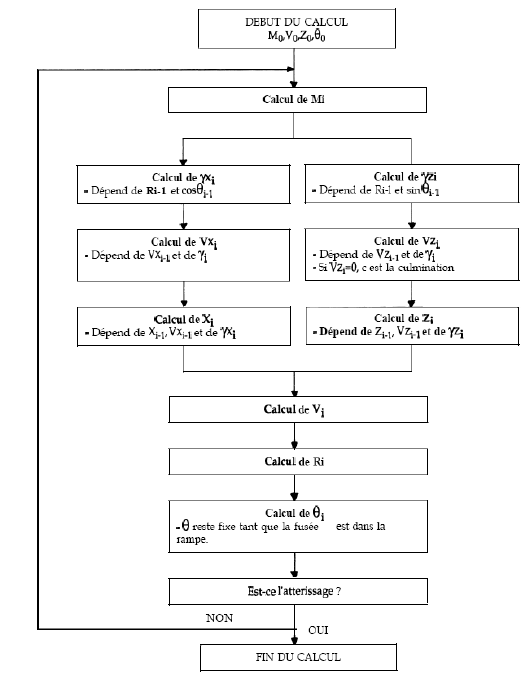
\includegraphics[width=9cm]{schema.PNG} 
\end{center}
\caption{Exemple pour le cas 2D.}
\label{scheme}
\end{figure}



\newpage

\part{Description du module Pégase}

Maintenant que l'essentiel de la théorie sur le vol de fusée a été présenté, cette partie aura pour vocation de décrire l'interface de calcul de et de simulation JAVA Pégase qui fait appelle a tout le bagages vu ci-dessus.\\



\section{Interface}


\begin{figure}[!htbp]
\begin{center}
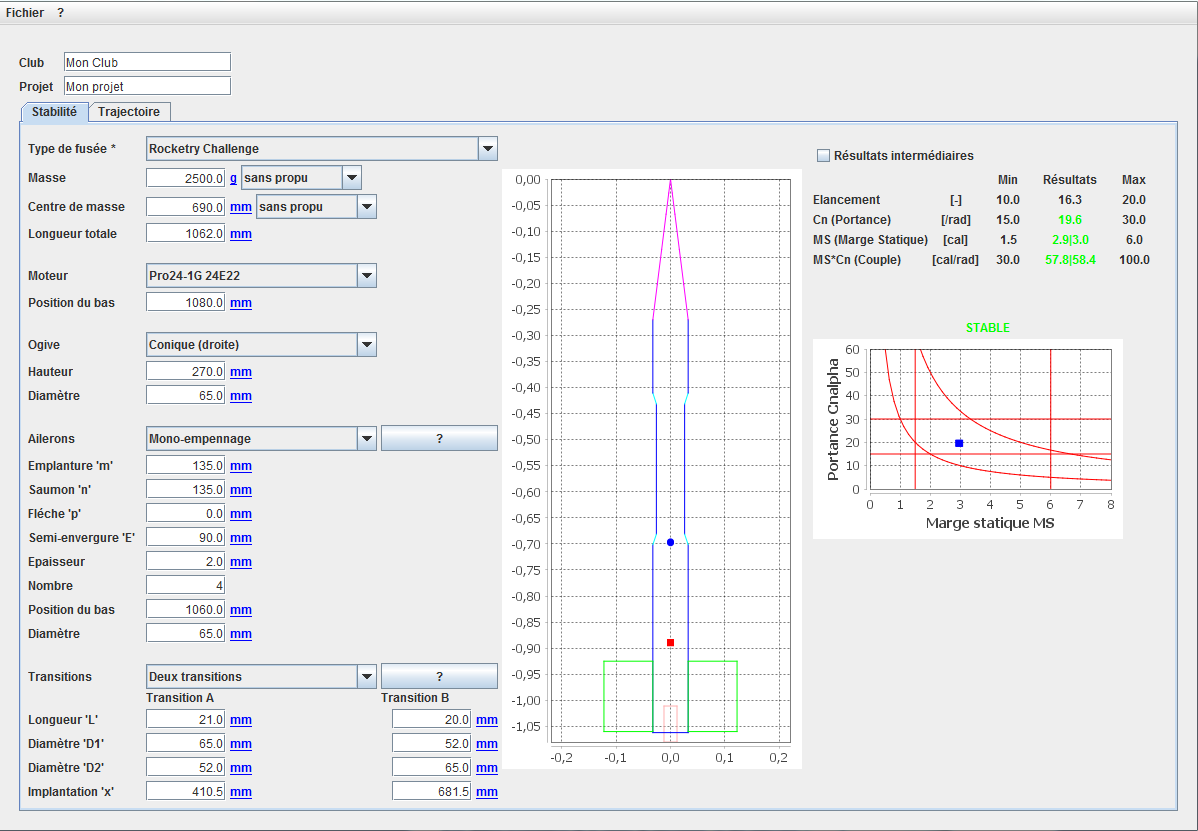
\includegraphics[width=11cm]{pegase.PNG} 
\end{center}
\caption{Interface Pégase - calcul de la stabilité.}
\label{peg1}
\end{figure}


L'interface de Pégase se divise en deux sections : un premier module pour le calcul de stabilité et un module pour le calcul de trajectoire 2D.


\begin{enumerate}
\item \textbf{Stabilité} : Dans cette section, l'utilisateur est invité à modéliser une fusée en entrant ses caractéristiques dans des cellules (\ref{peg1}). Une fois l'engin modélisé, Pégase stocke ces informations inputs et réalise les calculs afin de vérifier si la fusée vérifie les conditions de stabilité évoquées plus haut (marge statique, coefficient $C_{N}\alpha$ etc.) Au milieu de la fenêtre peut être observé un graphe représentant la fusée crée. À droite, un graphe de $C_{N}\alpha$ en fonction de la marge statique, indiquant si les caractéristiques sont dans le bon intervalle de stabilité \ref{peg1}.

\item \textbf{Trajectoire} : L'utilisateur doit entrer les inputs pour modéliser la phase de lancement via la rampe (hauteur, angle d'inclinaison, longueur etc.), le vitesse du vent pendant le vol  et les paramètre de la phase de parachute et le code de calcule s'occupe de tracer la trajectoire de la fusée.\\

À droite est représenté la trajectoire en fonction du temps et en fonction de l'axe des x \ref{peg2}. Juste en dessous sont affichés les informations calculés à des moments clés du vol (sortie de rampe, apogée, vitesse max etc.) \ref{peg2}.

\end{enumerate}


\begin{figure}[!htbp]
\begin{center}
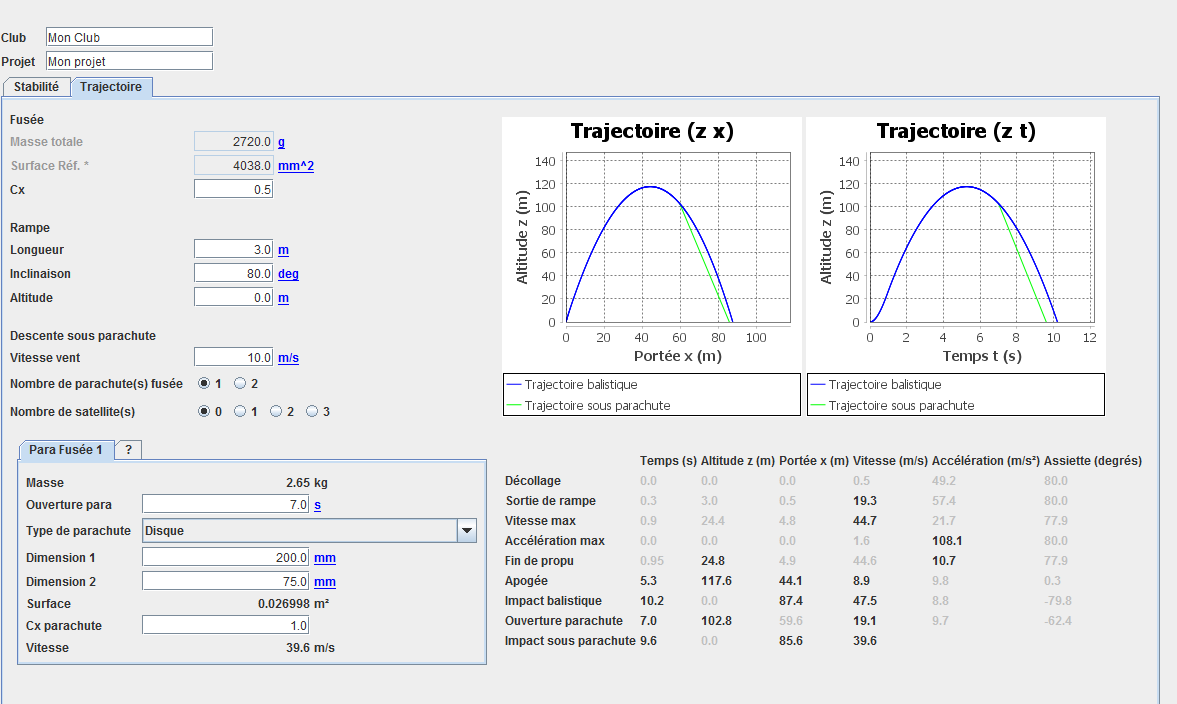
\includegraphics[width=11cm]{pegase2.PNG} 
\end{center}
\caption{Interface Pégase - calcul de la trajectoire.}
\label{peg2}
\end{figure}

L'algorithme classique pour le calcul de la trajectoire est inspiré de \ref{scheme} et est de la forme suivante :
\begin{verbatim}
\\Calcul des forces et accélérations 
M_i = M0 - dm.ti  \\nouvelle masse avec débit supposée constant dm
R_i  = (1/2)rho_i.C_Ai.S(V_i-1)^2  \\ Résistance de l'air
\\ P_i  = poussée à t_i calculée par la méthode getloidePoussée()

Gamma_xi = (P_i - R_i)/M_i . cos(theta_i-1)
Gamma_zi = (P_i - R_i)/M_i .sin(theta_i-1) - g

\\Calcul des vitesses
V_xi = (V_xi-1) + (Gamma_xi).dt_i	
V_zi = (V_zi-1) + (Gamma_zi).dt_i
V_i = ((V_xi)^2 + (V_zi)^2)^(1/2) \\norme vitesse à t_i

\\Calcul de la position et trajectoire
X_i = X_i-1 + (V_xi-1).dt_i +(1/2)(Gamma_xi).(dt_i)^2	\\selon x
Z_i = Z_i-1 + (V_zi-1).dt_i +(1/2)(Gamma_zi).(dt_i)^2	\\selon z

\\Màj de theta_i
a=tan(theta_i-1) = (V_zi)/(V_xi)
theta_i = arctan(a)

\end{verbatim}





Lorsque la composante verticale de la vitesse $V_{X_{i}}$ s'annule, la fusée est en phase de culmination.\\

Dans le cas ou la fusée est sur une rampe de lancement, il faut prendre en considération la hauteur à laquelle la fusée commence sa trajectoire, et l'angle d'inclinaison plus une force supplémentaire qui est la réaction {$\vec R$}. En adaptant le PFD, l'accélération à cette étape se calcul comme tel :
 
\begin{verbatim}

Gamma_xi = (P_i - R_i)/M_i.cos(theta_i)-g.cos(theta_i)sin(theta_i)
Gamma_zi = (P_i - R_i)/M_i.sin(theta_i)-g+g.cos(theta_i)^2	

\\avec theta_i = theta_0 l'angle formé par la rampe.

\end{verbatim}

On ne tient plus compte de la rampe de lancement lorsque l'altitude $Z_{i} - Z_{0}$ devient supérieure à L.sin($\theta_{0}$) (L est la longueur de la rampe).\\

Quand à la phase du parachute, sous l'action du poids et de la résistance de l'air seulement, la vitesse augmente ou diminue jusqu'à ce que la trainée égale le poids. L'accélération du mouvement étant alors nulle, la vitesse reste constante (vitesse limite $V_{l}$).
\begin{verbatim}
P = R   V = Cste = V_l 
M.g = (1/2).rho.S_para.C_x_para.V_l
V_l = (2.M.g/(rho.S_par.C_x_par))^(1/2)
\end{verbatim}


\section{Code}

Le code de Pégase est écrit en JAVA. Le paragraphe suivant va résumer l'essentiel des éléments de code générant l'interface.\\

Le code est basé autour de 3 classes principales :

\begin{verbatim}
class Fusee
class Stabilite
class Trajectoire	
\end{verbatim}


La première classe va permettre de modéliser la fusée et ses caractéristiques sont : son type, sa masse, la forme de son ogive etc.\\

La stabilité va dépendre du type auquel appartient la fusée. un calcul est fait pour vérifier si les inputs respectent bien les conditions de stabilités caractéristiques du type de fusée sélectionné.\\

\newpage

\begin{figure}[!htbp]
\begin{center}
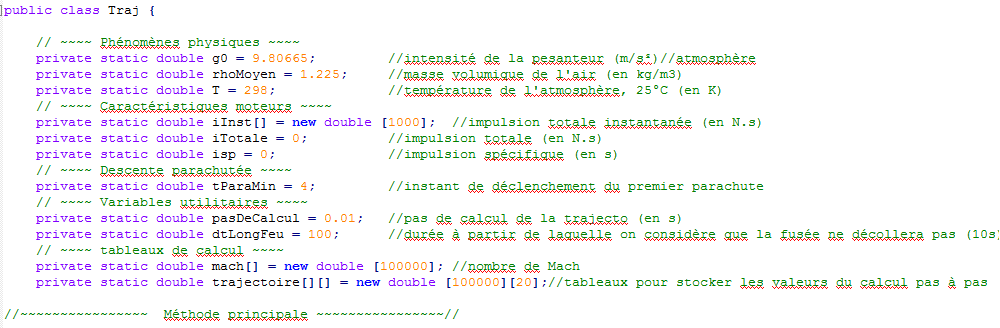
\includegraphics[width=15cm]{code.PNG} 
\end{center}
\caption{Extrait de code.}
\end{figure}

La trajectoire va être calculée à l'aide d'une classe. Les positions, vitesses et autres paramètres relatifs au vol de la fusée vont être stockés dans un tableau et les coordonnées de la position vont servir à tracer la trajectoire. Le schéma numérique utilisé et le même que celui décrit dans la partie précédente.



\section{Fusée multi-étagée}

L'interface Pégase ne réalise les calculs que pour les fusées mono étagées. Le cas des fusées multi-étagée est un peu différent dans la mesure ou il fait entrer d'autres paramètres en jeu : \\

\begin{itemize}
\item La fusée se sépare de ses étages à des moments données, entrainant un changement de masse et de géométrie.
\item Il faut par la suite considérer la stabilité et la trajectoire de chaque élément (étage) de la fusée.
\end{itemize}

Pour une fusée bi-étagée par exemple il faut considérer les configurations suivantes : 

\begin{enumerate}

\item[] Vol en configuration bi-étage,
\item[] Vol du second étage seul
\item[] Vol du premier étage seul

\end{enumerate}

Les changements de masse et de géométrie vont avoir un impact direct sur les forces mise en jeu et donc sur le schéma numérique modélisant la trajectoire.






\section{Conclusions}

Durant les prochains jours, on va tenter de formaliser la modélisation des fusée bi-étagée et l'étude de leur stabilité et trajectoire et enfin, d'inclure cela à l'interface de calcul Pégase.


%\bibliographystyle{plain}
%\bibliography{bibliography.bib}
\end{document}
